\documentclass[12pt,a4paper]{article}
\usepackage[a4paper, margin=0.8in]{geometry}
\usepackage{parskip}
\usepackage{titling}
\usepackage{graphicx}
\setlength{\droptitle}{-3em}

\begin{document}
    \section*{Database Schema}
    \subsection*{Table Definitions}
    \begin{center}
        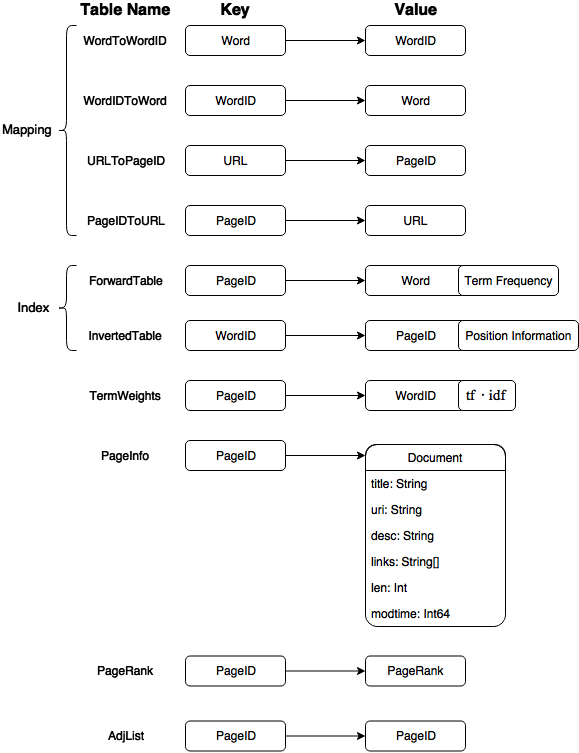
\includegraphics[scale=0.8]{databaseSchema} \\
    \end{center}

    \subsection*{Table Explanation}
    The database consists of several key/value tables that are stored locally on disk.
    The package used for our database manager is BoltDB, a persistent key/value storage for the Go programming language.
    BoltDB's underlying structure for the key/value table is B+ tree, and therefore our tables are implemented as B+ trees.

    As for the schema itself, the tables are grouped into four main categories:
    \begin{enumerate}
        \item Mappings \\
        Each word and page URL is represented by a 64-bit unique identifier.
        Four tables are used to maintain the mappings of ($word \leftrightarrow wordId$) and ($url \leftrightarrow pageId$), in which a single one-to-one relationship uses two tables for forward and inverse mapping.
        A separate table is created for the inverse mapping so that the lookup from an ID to its string representation can be done quickly without doing a linear search.
        Such lookup is done frequently when presenting the search results to the user.

        \item Indexes \\
        These tables form an integral part of our search functionality and consist of four tables: InvertedIndex and ForwardIndex for each title and body text.
        The indexes allow for both forward lookup ($pageId \rightarrow words$) and backward lookup ($wordId \rightarrow pages$).
        Title and body texts are put into separate indexes to allow different scoring for matches in the title and body.

        \item Scoring \\
        These tables contain scoring related information and must be updated after a set of pages has been added to the index.
        The scores are precomputed to allow faster retrieval.
        \begin{itemize}
            \item TermWeights stores the term weights ($tf \cdot idf$) of all terms in each page.
            \item AdjList stores the parent IDs of each page, along with the number of pages pointed by that parent.
            \item From this AdjList, the PageRank scores are precomputed, which are then stored in the table PageRank.
        \end{itemize}

        \item Page Metadata \\
        The page metadata only has one table, PageInfo, that stores the additional information such as title (unstemmed and contains stopwords) size, last-modified date, and child links.
        The metadata is not used to execute searches but is kept for the presentation of search results.

    \end{enumerate}



\end{document}